\section{Fault Tolerance}
\label{sec:ft}

We next introduce the fault tolerance mechanisms in \nfactor, for the controller, the virtual switch and the runtimes, respectively. 
Depending on the nature of these three components, we carefully design 
light-weighted replication mechanisms, targeting robustness and little impact on performance of their normal operations.

\subsection{Replicating Controller}

Since the controller is a single-threaded module that mainly collects the states of 
the runtimes, we persistently log these states and replicate them. The 
controller only needs to log the state of each runtime in 
the cluster view list. Whenever the controller needs to modify the state of a 
runtime, it logs the intended operation, modifies the state and logs a success 
mark for the intended operation.

The liveness of the controller is monitored by a guard process and the 
controller is restarted immediately in case of failure. On a reboot, the 
controller reconstructs the states in the cluster view list by replaying logs. 
Each runtime in the cluster monitors the connection status with the controller 
and reconnects to the controller in case of a connection failure.

\subsection{Replicating Virtual Switch}

The most important state of the virtual switch process is its switching hash 
table in memory. In order to replicate the virtual switch for failure resilience, we constantly 
check-point the container memory image of the virtual switch using CRIU 
\cite{criu}, a popular tool for checkpointing/restoring Linux processes. One main 
technical challenge is that CRIU has to stop a process before checkpointing it, 
which may hurt the availability of the virtual switch.

We tackle this challenge by letting the virtual switch call a 
fork() periodically (by default, one minute), and then we use CRIU to checkpoint 
the child process. Therefore, the virtual switch can proceed without affecting 
the system performance.

% Since the
% check-pointing needs to halt the execution of the whole virtual switch, it can
% not be frequently performed. In our implementation, we create a check-point for
% every second. However, this means that some states in the switching hash table
% might be lost and the flow connection related with these states may be forced to
% terminate. We argue that this is an acceptable implementation trade-off as flows
% could do a reconnection to complete unfinished tasks. If strong consistency is
% required, the virtual switch could use the replication strategy of
% FTMB\cite{sherry2015rollback}, we leave this to the future work.

\subsection{Replicating Runtime}

\begin{figure}
		\centering
		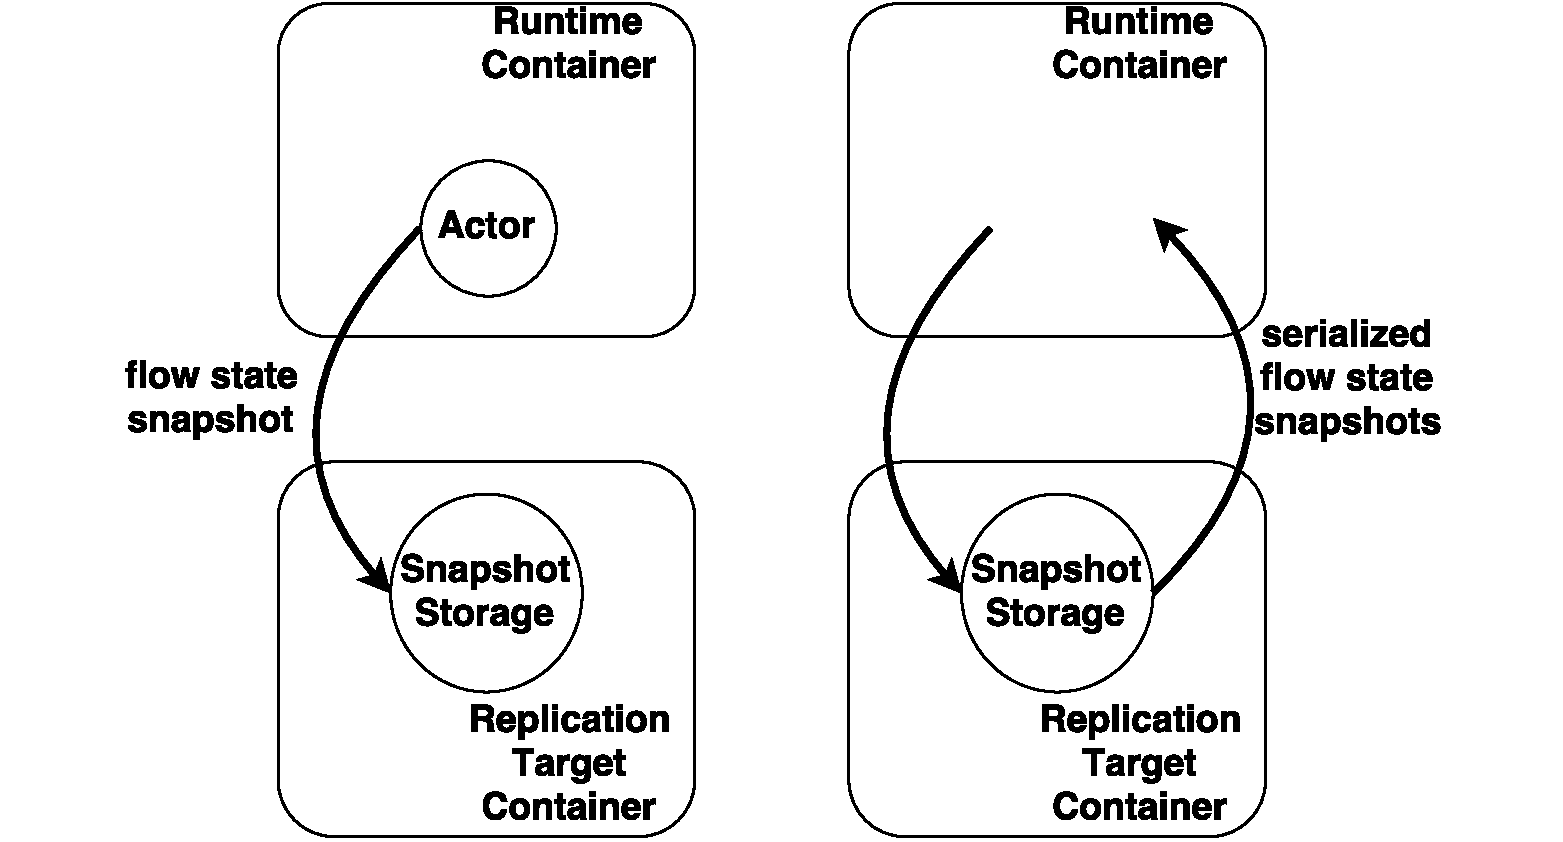
\includegraphics[width=\columnwidth]{figure/NFActor-Runtime-Replicate.pdf}

		\caption{Replication process used by for \nfactor~runtime. The left side figure illustrates how actor stores its flow state snapshots to the snapshot storage. The right side figure illustrates how recovered runtime fetches the snapshot storage from another runtime. }
\label{fig:replicate} 
\end{figure}

To perform lightweight runtime replication, we leverage the actor 
abstraction and state separation to create a lightweight flow state replication 
strategy. In a runtime, important flow states associated with a flow is 
owned by a unique actor. The runtime can replicate each actor 
independently without incurring the overhead of check-pointing the entire 
container images \cite{sherry2015rollback, rajagopalan2013pico}. In \nfactor, each actor replicates its state by choosing another runtime to store its flow state snapshots. This replication strategy avoids the need for using dedicated back-up servers \cite{sherry2015rollback} and achieves very good scalability, as newly created runtimes after scaling-out could also be used to store flow state snapshots.  

This primary-backup replication approach can tolerate the failure of one runtime (between runtimes that the actor and its replica are residing in. %actor failure at runtime. 
We think this fault-tolerance guarantee is sufficient because the 
chance for both runtimes (usually on two server machines) failing at the same time is extremely low.

\textbf{Finding a Replication Target}: When an actor is created, it selects a runtime in the
\textit{running} state with the smallest workload as its replication
target. Then the actor negotiates with the replication target about whether the
replication target can accept this actor's flow state snapshot. In case that replication
target refuses to store the actor's state snapshot, the actor tries to select
another replication target. 

\textbf{Snapshot Storage}: Each runtime maintains several snapshot storage for each runtime in the cluster except itself. The snapshot storage stores all the flow state snapshots sent from the same runtime. Each snapshot storage is managed by an independent thread for fast storing and retrieving.

\textbf{Flow State Replication (Fig.~\ref{fig:replicate})}: After determining
the replication target, the actor performs flow state replication. For every fixed number of packets that the actor has processed, the actor creates a
snapshot of the flow states of all NF modules and sends the snapshot to the snapshot storage on the actor's replication target. Note that the flow state replication is independent with NF processing and it ensures built-in fault tolerance. The snapshot storage keeps saving the newly received snapshot and discarding the old one. Note that this replication strategy only ensures weak consistency because once the runtime fails, the actors on the failed runtime can only be recovered to its old state. For strong consistency, NFActor could be easily extended to a similar framework as in \cite{sherry2015rollback}. However, as we can see from Sec. \ref{sec:rp}, even using replication with weak consistency imposes a significant overhead on the performance of the NFActor runtimes.

%The replica keeps saving the content (processed packet, state snapshot) of the received replication message in memory. If the received message includes a new state snapshot, the replica wipes out all previously saved content to decrease memory usage. Finally, the replication target sends the input packet copy out from its output port to the virtual switch. This replication procedure ensures that the same output commit property as indicated in \cite{sherry2015rollback}, as the receiver side of the flow can only observe output packets that are correctly logged \chuan{explain more of the idea why both original actor and the replica need to send the output packet to the virtual switch}. 

\textbf{Recovering Failed Runtime (Fig.~\ref{fig:replicate})}: In case that a runtime fails, the controller will immediately detect the failure and reboot the failed runtime. The restarted runtime first performs recovery process by sending a recovery message to every other runtime in the cluster, asking for content of the snapshot storage of the recovered runtime. The recovered runtime then uses these snapshot storage to reconstruct its flow states before failure. The reconstruction process could be paralleled on different threads because each snapshot storage could be used independently.  When the runtime finishes recovery, it re-joins the cluster and resumes normal flow processing. 

%\chuan{Increase font size in Fig. 4.}

% \textbf{Discussion}: The runtime replication strategy can tolerate at most one
% failed runtime. If multiple runtimes fail concurrently, then the replicas will
% be lost and the states of some flows will never be correctly recovered.
% Multi-machine replication algorithm such as PAXOS \cite{chandra2007paxos} could
% be used to replicate the flow state to multiple backups. However, PAXOS may not
% be efficient enough to handle the replication of a large number of packets. We
% leave exploring multi-backup to our future work. 


